\begin{enumerate}
	\item \textbf{Check National Number Votes}
		\begin{enumerate}
			\item \textbf{Service Contract}
				\begin{figure}[H]
					\centering
					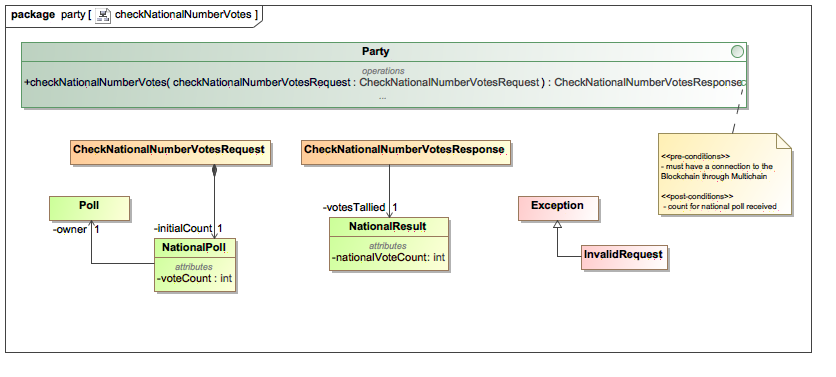
\includegraphics[width=0.75\linewidth]{../Images/Party/ServiceContracts/CheckNationalNumberVotes_ServiceContract.png}
					\caption{Check National Number Votes Service Contract}
				\end{figure}
				
				\begin{enumerate}
					\item Pre-conditions
					\begin{itemize}
						\item There must be a connection to the Blockchain through the Multichain
					\end{itemize}
					
					\item Exceptions
					\begin{itemize}
						\item If there is no connection to the Blockchain, the InvalidRequest exception will be thrown
					\end{itemize}
					
					\item Post-conditions
					\begin{itemize}
						\item The count for the National Poll is received
					\end{itemize}
				\end{enumerate}
			
			\item \textbf{Functional Requirements}
				\begin{figure}[H]
					\centering
					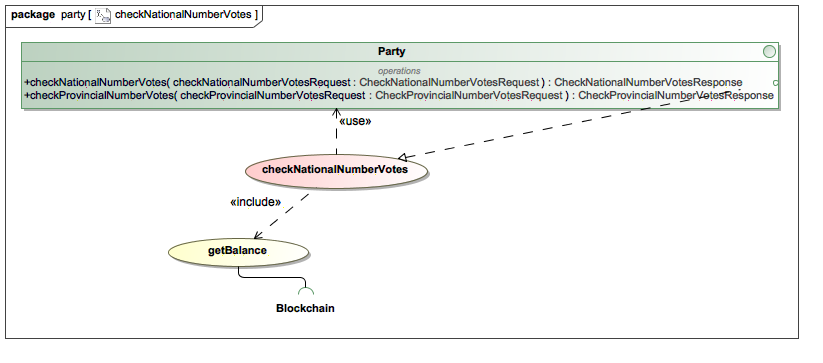
\includegraphics[width=0.75\linewidth]{../Images/Party/UseCases/CheckNationalNumberVotes_UseCase.png}
					\caption{Check National Number Votes Use Case}
				\end{figure}
				
				\newpage
				
			\item \textbf{Process Design}
				\begin{figure}[H]
					\centering
					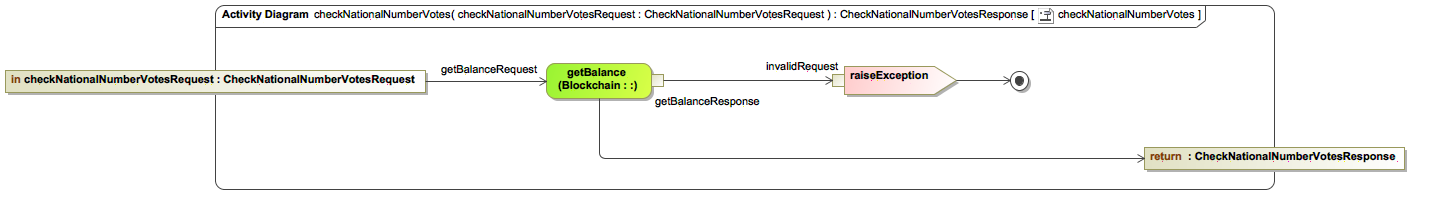
\includegraphics[width=0.75\linewidth]{../Images/Party/ActivityDiagrams/CheckNationalNumberVotes_Activity.png}
					\caption{Check National Number Votes Activity}
				\end{figure}
				
		\end{enumerate}
	
	\item \textbf{Check National Number Votes}
		\begin{enumerate}
			\item \textbf{Service Contract}
			\begin{figure}[H]
				\centering
				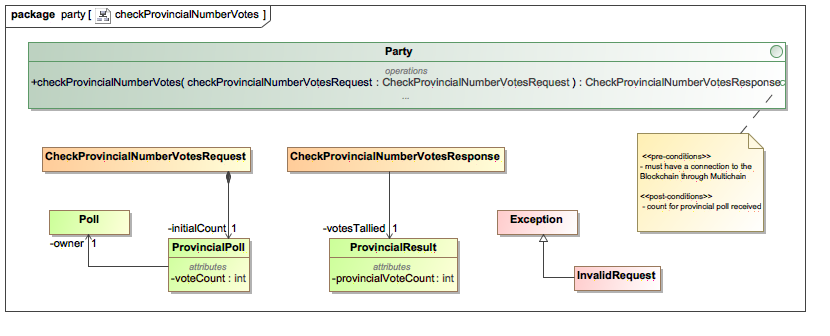
\includegraphics[width=0.75\linewidth]{../Images/Party/ServiceContracts/CheckProvincialNumberVotes_ServiceContract.png}
				\caption{Check National Number Votes Service Contract}
			\end{figure}
			
			\begin{enumerate}
				\item Pre-conditions
				\begin{itemize}
					\item There must be a connection to the Blockchain through the Multichain
				\end{itemize}
				
				\item Exceptions
				\begin{itemize}
						\item If there is no connection to the Blockchain, the InvalidRequest exception will be thrown
				\end{itemize}
				
				\item Post-conditions
				\begin{itemize}
					\item The count for the Provincial Poll is received
				\end{itemize}
			\end{enumerate}
			
			\item \textbf{Functional Requirements}
			\begin{figure}[H]
				\centering
				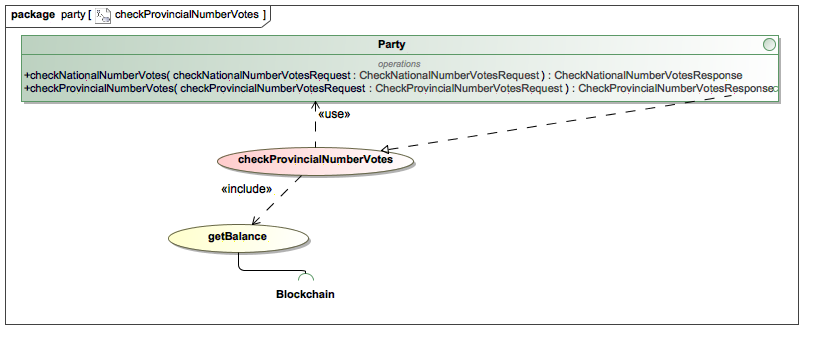
\includegraphics[width=0.75\linewidth]{../Images/Party/UseCases/CheckProvincialNumberVotes_UseCase.png}
				\caption{Check National Number Votes Use Case}
			\end{figure}
						
			\item \textbf{Process Design}
			\begin{figure}[H]
				\centering
				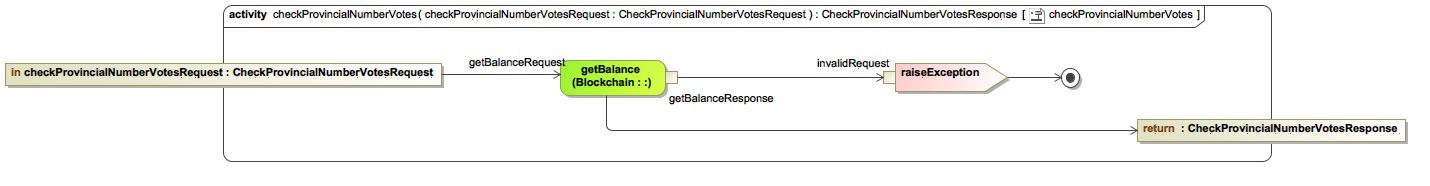
\includegraphics[width=0.75\linewidth]{../Images/Party/ActivityDiagrams/CheckProvincialNumberVotes_Activity.png}
				\caption{Check National Number Votes Activity}
			\end{figure}
			
		\end{enumerate}
\end{enumerate}